\documentclass[11pt]{article}
\usepackage[margin=1in]{geometry}
\usepackage{amsmath,amssymb,amsthm}
\usepackage{mathptmx}
\usepackage{booktabs,graphicx}
\usepackage[authoryear,round]{natbib}
\usepackage[colorlinks=true,citecolor=blue,linkcolor=blue,urlcolor=blue]{hyperref}
\setlength{\emergencystretch}{2em}
\linespread{1.1}

\theoremstyle{plain}
\newtheorem{theorem}{Theorem}
\newtheorem{proposition}{Proposition}
\newtheorem{lemma}{Lemma}
\newtheorem{corollary}{Corollary}
\theoremstyle{definition}
\newtheorem{example}{Example}
\theoremstyle{remark}
\newtheorem{remark}{Remark}

\newcommand{\E}{\mathbb E}
\newcommand{\R}{\mathbb R}
\newcommand{\ind}{\mathbf 1}
\DeclareMathOperator{\clip}{clip}
\DeclareMathOperator{\sgn}{sgn}
\DeclareMathOperator{\dist}{dist}
\DeclareMathOperator{\logit}{logit}

\title{Learning Wavelet Shrinkage from Noisy Labels: 
Stein Calibration with Interval Teachers}
\author{  Vijini Lakmini$^{1}$, Dixon Vimalajeewa$^{2}$,  and Brani Vidakovic$^{1}$ \\
\\
{\small $^{1}$Department of Statistics, Texas A\&M University, College Station, TX 77843, USA} \\
\small $^{2}$ Department of Statistics, University of Nebraska, Lincoln, NE 68588, USA}
 

\date{Draft 06}

\begin{document}
\maketitle

\begin{abstract}
Two-threshold wavelet shrinkage leaves coefficients of intermediate magnitude undecided, and
\emph{MLShrink} resolves them with a trained classifier. We study what such a classifier
should learn when its labels are themselves uncertain. The decision is framed as a choice, or
an interpolation, between two shrinkage rules. Gaussian integration by parts turns each
coefficient into an unbiased score for the reconstruction cost of moving between the rules, and
a gate that depends only on neighbouring and parent coefficients is fitted by a convex quadratic
Stein objective with an explicit population target. Noisy labels enter through partial
identification. When the flip probabilities of a binary label are unknown but bounded, the
noisy-label probability determines a sharp interval for the clean probability at each feature
value. For labels of slab membership this becomes an interval of shrinkage actions whose
midpoint minimizes the worst-case conditional regret; for labels that record which rule wins,
no interval of probabilities determines the sign of the expected cost. We propose
interval-teacher calibration, which penalizes the squared distance of the Stein gate from a
label-derived interval. The fit remains convex, and for piecewise-constant gates a realized
interval that contains the population target of a cell cannot increase the risk of that cell,
for every training sample and every penalty weight. In simulations with estimated intervals,
the interval teacher removed most of the excess risk of the Stein gate when training data were
scarce and was worse than no teacher in at most 1.5\% of replicates. A point teacher gained more
when its target was accurate, but under one-sided label noise it was worse than no teacher in up
to half of the replicates even with a cross-fitted penalty. Two wavelet experiments illustrate
both kinds of label.
\end{abstract}

\section{Introduction}\label{sec:intro}

Wavelet shrinkage estimates a signal by transforming noisy observations, modifying the
empirical coefficients, and inverting the transform
\citep{donoho1995adapting}. Most rules decide the fate of a coefficient from its magnitude,
possibly calibrated by a prior \citep{abramovich1998wavelet,clyde1998multiple,
vidakovic2001bams,johnstone2005empirical}, and a second line of work lets neighbouring and
parent coefficients inform the decision \citep{crouse1998wavelet,cai2001incorporating,
sendur2002bivariate}. \emph{MLShrink} \citep{vimalajeewa2026mlshrink} combines the two
ideas: coefficients below a lower threshold are discarded, those above an upper threshold
are kept, and a classifier using local context decides the coefficients in between.

The classifier must be trained, and its labels are never the quantity that governs
reconstruction error. Labels produced by the thresholds are deterministic functions of the
coefficient magnitude; labels computed from clean training signals depend on the
unobserved noise; and labels supplied by detectors, annotators or auxiliary channels are
corrupted in ways that are rarely known exactly. The literature on learning with noisy
labels offers a rich set of tools for such problems, from consistency theory under
class-conditional noise \citep{natarajan2013learning,scott2013classification,
menon2015learning,blanchard2016classification,cannings2020classification} to loss
correction and sample selection for deep networks \citep{patrini2017making,
han2018coteaching,song2023learning}. These tools, however, target classification accuracy,
whereas shrinkage is judged by squared error, and the cost of a wrong decision varies from
coefficient to coefficient.

This paper takes the cost as primary and treats labels as auxiliary information about
which actions are plausible. We generalize the keep-or-discard decision to a choice between
two shrinkage rules, and to interpolation between them, so that hard thresholding, soft
thresholding and Bayesian posterior means are covered by one formulation. Stein's identity
\citep{stein1981estimation} then provides, for every coefficient, an unbiased score of the
cost of moving from one rule to the other, without any label. A gate that depends only on
context is fitted by minimizing Stein's unbiased risk estimate, which is a convex quadratic
in the gate, and the population minimizer is explicit. The role of noisy labels is to
regularize this fit. When the flip probabilities of a label are unknown but bounded, the
label does not identify the clean probability; it identifies an interval for it, in the
sense of partial identification \citep{manski2003partial}. We show that this interval is
sharp at each feature value, that for labels of slab membership it translates into an
interval of shrinkage actions with a minimax midpoint, and that for labels recording which
rule wins it does not determine the sign of the expected cost at all. The proposed
interval-teacher calibration uses the label-derived interval as a soft constraint on the
Stein gate. Its main property is conditional: for piecewise-constant gates, an interval that
contains the population target can only help, since the penalized fit is never farther from
that target, and never has larger risk, than the unpenalized fit, whatever the training sample
and the penalty weight. Whether an estimated interval contains the target is a separate,
probabilistic question, which we examine empirically.

\paragraph{Related work.} Learning from corrupted labels was formalized for random
classification noise by \citet{angluin1988learning}, and early statistical treatments built
the flipping process into the likelihood \citep{lawrence2001estimating,bootkrajang2012label}.
Under class-conditional noise, unbiased surrogate losses \citep{natarajan2013learning},
shifted thresholds for class-probability estimates \citep{menon2015learning} and importance
reweighting \citep{liu2016classification} are consistent, and unknown asymmetric rates are
identifiable under irreducibility conditions linked to mixture-proportion estimation
\citep{scott2013classification,blanchard2016classification,ramaswamy2016mixture}; the
transition matrix is not identifiable in general \citep{liu2023identifiability}.
\citet{cannings2020classification} and \citet{reeve2019fast} show which standard classifiers
remain consistent with imperfect labels. For deep networks, which can fit arbitrary labels
\citep{zhang2017understanding,arpit2017closer}, the main responses are loss correction
\citep{patrini2017making,hendrycks2018using}, robust losses \citep{ghosh2017robust,
zhang2018generalized,wang2019symmetric}, selection and reweighting of examples
\citep{han2018coteaching,jiang2018mentornet,ren2018learning,shu2019meta}, semi-supervised
treatment of suspect labels \citep{li2020dividemix}, early-learning regularization
\citep{liu2020early} and data cleaning \citep{northcutt2021confident}; surveys are
\citet{frenay2014classification}, \citet{han2020survey}, \citet{algan2021image} and
\citet{song2023learning}. Instance-dependent noise, the case relevant here, is treated by
\citet{xia2020part} and \citet{cheng2021learning}. Self-supervised denoising trains on noisy
targets by design \citep{lehtinen2018noise2noise,batson2019noise2self,krull2019noise2void,
moran2020noisier2noise,pang2021recorrupted}, and it is the counterpart, for learned
denoisers, of the Stein calibration used below. What distinguishes the present setting is
that the loss is squared reconstruction error, so the relevant target is a cost rather than
a class, and that the noisy labels are used to bound, rather than to estimate, the quantity
they describe.

Section~\ref{sec:setting} sets up the two-rule decision and explains why the label of the
winning rule, and labels produced by thresholds, are inadequate targets.
Section~\ref{sec:interval} introduces the interval of actions and its oracle.
Section~\ref{sec:stein} develops Stein calibration of context gates.
Section~\ref{sec:labels} characterizes what noisy labels identify.
Section~\ref{sec:teacher} presents interval-teacher calibration and its guarantees.
Section~\ref{sec:simplan} reports a known-prior simulation, Section~\ref{sec:waveplan}
reports two wavelet experiments built on BAMS, and
Section~\ref{sec:discussion} discusses limitations. Margin bounds for binary rules are given
in Appendix~\ref{app:margin}; an analysis of recorruption, an alternative to Stein scores when
a learner is not differentiable, is given in the Supplementary Material.

\section{Shrinkage between two rules}\label{sec:setting}

\subsection{Model and cost contrast}

We work with an orthonormal wavelet transform, so that the empirical detail coefficients
satisfy $D=\theta+\sigma Z$ with $Z\sim N(0,I_n)$, and Parseval's identity transfers total
squared error between the coefficient and signal domains. Stein identities are stated for
fixed $\theta$ and known $\sigma$; statements about posterior means additionally treat
$\theta$ as random and independent of $Z$. For coordinate $i$ let $X_i=(D_i,U_i)$, where
the context $U_i$ may contain the level, same-scale neighbours and the parent coefficient.
Whenever $U_i$ is built from coefficients other than $D_i$, it is independent of $Z_i$.

Let $A_i$ and $C_i$ be two shrinkage rules evaluated at $X_i$, with $A_i$ the stronger. Put
$B_i=C_i-A_i$ and $M_i=(A_i+C_i)/2$. The reduction in squared error obtained by using $C_i$
rather than $A_i$ is
\begin{equation}\label{eq:contrast}
r_i=(A_i-\theta_i)^2-(C_i-\theta_i)^2=2B_i(\theta_i-M_i),
\end{equation}
and the label of the winning rule is $L_i^\star=\ind\{r_i\ge0\}$. With
$m_i(X_i)=\E(\theta_i\mid X_i)$, the conditional expected contrast is
$g_i(X_i)=2B_i\{m_i(X_i)-M_i\}$, and the Bayes binary rule selects $C_i$ exactly when
$g_i\ge0$. The keep-or-discard decision of \emph{MLShrink} is the case $(A_i,C_i)=(0,D_i)$,
for which $r_i=2D_i\theta_i-D_i^2$.

\subsection{Which label should be learned}

\begin{lemma}[Cost weighting]\label{lem:cost}
Unweighted classification of $L_i^\star$ targets $P(r_i\ge0\mid X_i)$, which compares a
conditional median of $\sgn(B_i)\theta_i$ with $\sgn(B_i)M_i$. Classification with weights
$|r_i|$ and a classification-calibrated loss, or least-squares regression of $r_i$ on
$X_i$, recovers the sign of $g_i$ and hence the Bayes binary rule.
\end{lemma}

\begin{proof}
By \eqref{eq:contrast}, $r_i\ge0$ if and only if $\sgn(B_i)(\theta_i-M_i)\ge0$, which gives
the first statement. With weights $|r_i|$, the effective class masses at $X_i$ are
$\E\{(r_i)_+\mid X_i\}$ and $\E\{(r_i)_-\mid X_i\}$, whose difference is $g_i$; a calibrated
loss selects the class with the larger mass \citep{elkan2001foundations,scott2012calibrated}.
The regression function of $r_i$ is $g_i$.
\end{proof}

Because a spike-and-slab posterior is typically bimodal and skewed on the undecided band,
its median and its mean can lie on opposite sides of $M_i$; perfectly observed winning
labels can therefore lead to the wrong decision.

\begin{example}\label{ex:median}
Take the keep-or-discard pair $(A_i,C_i)=(0,D_i)$, so that $M_i=D_i/2$, and the centred
Gaussian spike-and-slab prior of Section~\ref{sec:interval} with $\sigma=1$, $\tau=3$ and
inclusion probability $\pi=0.45$. At $D_i=2$ the shrinkage factor is $s=0.9$ and the posterior
inclusion probability is $w_\pi(2)=0.610$. The posterior mean is $m_i=s\,w_\pi(2)\,D_i=1.098$,
which exceeds $M_i=1$, so keeping is the Bayes decision, with $g_i=2D_im_i-D_i^2=0.39>0$.
The slab part of the posterior is $N(1.8,0.9)$, which places probability $0.80$ above $1$,
so $P(L_i^\star=1\mid D_i)=0.610\times0.80=0.488<1/2$: a majority of perfectly observed winner
labels would discard the coefficient. The posterior mass at zero pulls the median below
$M_i$, while the slab mass far above $M_i$ pulls the mean above it.
\end{example}

Labels produced by the thresholds are worse still.

\begin{proposition}[Same-view threshold labels]\label{prop:leak}
Suppose the training set consists of coefficients outside an undecided band
$\{\lambda_1<|D_i|<\lambda_2\}$ with labels $\ind\{|D_i|\ge\lambda_2\}$, and $|D_i|$ is a
feature. Then on the training support the label is a deterministic function of $|D_i|$,
every consistent learner converges there to a function of $|D_i|$ alone, and its decisions
inside the band are determined by its inductive bias rather than by the labels.
\end{proposition}

\begin{proof}
On the training support $P(\text{label}=1\mid X_i)=\ind\{|D_i|\ge\lambda_2\}$, which does
not depend on $U_i$, and the band is a gap in that support.
\end{proof}

Such labels cannot teach how context should change a decision, and inverting a noise model
does not help, since their flip behaviour is degenerate on the support of the features
\citep{natarajan2013learning,liu2023identifiability}. The rest of the paper replaces them by
a cost score and uses genuinely external labels only as side information.

\section{An interval of actions}\label{sec:interval}

For a gate $p_i\in[0,1]$, consider the action $\delta_i=A_i+B_ip_i$, which interpolates
between the two rules. Two families of endpoints are used below. The first consists of soft
thresholds $A_i=S_{\lambda_2}(D_i)$ and $C_i=S_{\lambda_1}(D_i)$, with
$S_\lambda(d)=\sgn(d)(|d|-\lambda)_+$ and $0\le\lambda_1<\lambda_2$; they agree below
$\lambda_1$, differ by a constant magnitude above $\lambda_2$, and have weak derivatives
$\ind\{|D_i|>\lambda\}$. The second consists of Bayes rules. Under the centred Gaussian
spike-and-slab prior with inclusion probability $\pi$ and slab variance $\tau^2$, the
posterior mean is $s\,w_\pi(d)\,d$, where $s=\tau^2/(\tau^2+\sigma^2)$ and
\begin{equation}\label{eq:wpi}
w_\pi(d)=\frac{\pi\,\phi_{\sigma_1}(d)}{\pi\,\phi_{\sigma_1}(d)+(1-\pi)\,\phi_\sigma(d)},
\qquad \sigma_1^2=\sigma^2+\tau^2,
\end{equation}
is the posterior inclusion probability, with $\phi_v$ the $N(0,v^2)$ density. Since
$w_\pi(d)$ increases in $\pi$, the choice $A_i=s\,w_{\pi_{\rm lo}}(D_i)D_i$ and
$C_i=s\,w_{\pi_{\rm hi}}(D_i)D_i$ with $\pi_{\rm lo}<\pi_{\rm hi}$ gives ordered endpoints. In
both families $0\le A_i/D_i\le C_i/D_i\le1$ for $D_i\ne0$, so every interpolated action
preserves sign and satisfies $|\delta_i|\le|D_i|$. When the original zero and identity
branches of \emph{MLShrink} are to be kept, the continuous bridge
$d\,v\,e^{f(X)}/\{1-v+v\,e^{f(X)}\}$ with
$v=\clip\{(|d|-\lambda_1)/(\lambda_2-\lambda_1),0,1\}$ and bounded, locally absolutely
continuous $f$ matches both branches at the thresholds. A hard switch between unequal
endpoint values would require boundary corrections in Stein's identity, and a band
indicator must never be treated as fixed when Stein's lemma is applied to a discontinuous
rule.

\begin{proposition}[Oracle interpolation]\label{prop:oracle}
Given $X_i$, the action in the closed interval with endpoints $A_i$ and $C_i$ that
minimizes conditional squared error is the projection of $m_i$ onto that interval. The best
endpoint has additional conditional risk $\ind\{0<t_i<1\}B_i^2\min(t_i,1-t_i)^2$, where
$t_i=(m_i-A_i)/B_i$ and the expression is zero when $B_i=0$; the improvement of
interpolation is strict in total risk whenever $P(B_i\ne0,\,0<t_i<1)>0$ for some $i$. For a
plug-in conditional mean $\widehat m_i$ fitted independently of the test coordinate, the
excess risk of its projected action is at most
$\E\{(\widehat m_i-m_i)^2\ind(B_i\ne0)\}$.
\end{proposition}

\begin{proof}
Conditional squared error equals the posterior variance plus the squared distance to $m_i$.
Outside the interval both oracles choose the same endpoint; inside, the projection has
distance zero and the nearest endpoint has distance $|B_i|\min(t_i,1-t_i)$. For the plug-in
claim let $q$ and $\widehat q$ be the projections of $m_i$ and $\widehat m_i$. The
projection inequality $(\widehat m_i-\widehat q)(q-\widehat q)\le0$ gives
$(\widehat q-m_i)^2-(q-m_i)^2\le2(\widehat m_i-m_i)(\widehat q-q)-(\widehat q-q)^2
\le(\widehat m_i-m_i)^2$, and the excess vanishes when the interval is a singleton.
\end{proof}

For $(A_i,C_i)=(0,D_i)$ the oracle is the soft rule $D_i\clip(m_i/D_i,0,1)$, which dominates
every keep-or-discard rule. Strict oracle dominance does not imply that a fitted soft rule
improves on a fitted binary rule, which is why the fitting procedure matters.

\section{Stein calibration of context gates}\label{sec:stein}

Write $\partial_i$ for differentiation with respect to $D_i$ with the other coefficients
held fixed. For a rule $\delta$ that is coordinatewise absolutely continuous with integrable
derivatives, Stein's unbiased risk estimate is
\begin{equation}\label{eq:sure}
\mathcal S(\delta)=\|\delta-D\|^2+2\sigma^2\sum_i\partial_i\delta_i-n\sigma^2,
\end{equation}
which is unbiased for $\E\|\delta-\theta\|^2$ at any fixed tuning
\citep{stein1981estimation,donoho1995adapting}. Minimizing $\mathcal S$ over a family and
reporting the minimum as the risk of the selected rule introduces selection bias; risks
are therefore assessed on independent data throughout.

Let the gate depend on context only, $p_i=p(U_i)$, so that $\partial_ip_i=0$, while the
endpoints may depend on $(D_i,U_i)$. Define the Stein score and weight
\begin{equation}\label{eq:score}
Y_i=B_i(D_i-A_i)-\sigma^2\partial_iB_i,\qquad V_i=B_i^2 .
\end{equation}

\begin{proposition}[Stein score]\label{prop:score}
For a context-only gate,
\begin{equation}\label{eq:quadratic}
\mathcal S(A+Bp)-\mathcal S(A)=\sum_i\bigl(V_ip_i^2-2Y_ip_i\bigr),
\end{equation}
and $\E(Y_i\mid U_i)=\E\{B_i(\theta_i-A_i)\mid U_i\}$. With
$z(U)=\E(Y\mid U)/\E(V\mid U)$, the population context-only gate is
$p^\star(U)=\clip\{z(U),0,1\}$ wherever $\E(V\mid U)>0$, and the conditional excess risk of
any gate value $p$ is
\begin{equation}\label{eq:excess}
\E(V\mid U)\bigl\{(p-p^\star)^2+2(p-p^\star)(p^\star-z)\bigr\},
\end{equation}
in which the second term is nonnegative and vanishes when $p^\star$ is interior.
\end{proposition}

\begin{proof}
Expanding \eqref{eq:sure} with $\partial_i(A_i+B_ip_i)=\partial_iA_i+p_i\partial_iB_i$ gives
\eqref{eq:quadratic}. Conditionally on $U_i$, $D_i$ is Gaussian with mean $\theta_i$ and
variance $\sigma^2$, so Stein's lemma gives $\E\{B_i(D_i-\theta_i)\mid U_i\}
=\sigma^2\E(\partial_iB_i\mid U_i)$, hence the score identity; under a prior the same
holds by iterated expectation. The conditional risk of $p$ equals a constant plus
$\E(V\mid U)\{(p-z)^2-z^2\}$, whose minimizer over $[0,1]$ is the clipped value, and
expanding $(p-z)^2-(p^\star-z)^2$ gives \eqref{eq:excess}. The cross term is nonnegative by
the projection property of $p^\star$.
\end{proof}

The score $Y_i$ is an unnormalized, label-free target: it involves neither a hard threshold
nor division by $B_i$, and \eqref{eq:excess} shows that gate errors are weighted by the
expected separation $\E(V\mid U)$ of the two rules. With features $\psi_i$ formed from
context and an affine gate $p_i=\psi_i^{\mathsf T}\beta$, where the $\psi_i$ are nonnegative,
bounded and sum to one and $\beta\in[0,1]^K$, the empirical objective
$\sum_i(V_ip_i^2-2Y_ip_i)$ is a convex quadratic in $\beta$ with Hessian
$2\sum_iV_i\psi_i\psi_i^{\mathsf T}$, and its population version is the $\E(V\mid U)$-weighted
least-squares projection of $z$ onto the gate class. Ridge penalties and fixed-weight
parent--child penalties $\gamma\sum_{(i,j)}w_{ij}(p_i-p_j)^2$ preserve convexity. Learned
combinations of elementary denoisers by SURE have precedents in SURE-LET
\citep{luisier2007sure}; the use of the endpoint score here is to calibrate supervision
within a prescribed interval of actions.

\paragraph{Point teachers.} A model-assisted teacher $q(U)\in[0,1]$, frozen before
evaluation, can be used as a shrinkage target by adding $\omega\sum_iV_i(p_i-q_i)^2$ to
\eqref{eq:quadratic}. For a context-only teacher the conditional optimum is
\begin{equation}\label{eq:pointteacher}
p_\omega=\clip\Bigl\{\frac{z+\omega q}{1+\omega},0,1\Bigr\},
\end{equation}
so that $\omega=0$ targets the Stein oracle and $\omega>0$ stabilizes the fit at the price
of a bias of size $\omega|q-z|/(1+\omega)$ whenever the teacher differs from the target.
Section~\ref{sec:teacher} replaces the point by an interval and removes this bias whenever
the interval is correct.

\section{What noisy labels identify}\label{sec:labels}

\subsection{Bounded instance-dependent noise}

Let $L\in\{0,1\}$ be a clean label with $\eta(x)=P(L=1\mid x)$, and let $\widetilde L$ be an
observed label with $\widetilde\eta(x)=P(\widetilde L=1\mid x)$ and instance-dependent flip
probabilities $\rho_0(x)=P(\widetilde L=1\mid L=0,x)$ and $\rho_1(x)=P(\widetilde L=0\mid
L=1,x)$ \citep{frenay2014classification,xia2020part}. Conditioning on $L$ gives
\begin{equation}\label{eq:noisemodel}
\widetilde\eta(x)=\rho_0(x)\{1-\eta(x)\}+\{1-\rho_1(x)\}\eta(x).
\end{equation}
With known rates this identity can be inverted \citep{natarajan2013learning,
menon2015learning}. In applications the rates are rarely known, but an analyst may be able
to defend upper bounds on them.

\begin{proposition}[Sharp bounds on the clean probability]\label{prop:bracket}
Suppose $0\le\rho_0(x)\le\bar\rho_0(x)$ and $0\le\rho_1(x)\le\bar\rho_1(x)$ with
$\bar\rho_0(x)+\bar\rho_1(x)<1$, and define
\begin{equation}\label{eq:bracket}
\eta_-(x)=\clip\Bigl\{\frac{\widetilde\eta(x)-\bar\rho_0(x)}{1-\bar\rho_0(x)},0,1\Bigr\},
\qquad
\eta_+(x)=\clip\Bigl\{\frac{\widetilde\eta(x)}{1-\bar\rho_1(x)},0,1\Bigr\}.
\end{equation}
Then $\eta_-(x)\le\eta(x)\le\eta_+(x)$ for every $x$. The bounds are sharp at each $x$: the
lower bound is attained with $\rho_1(x)=0$ and $\rho_0(x)=\min\{\bar\rho_0(x),
\widetilde\eta(x)\}$, and the upper bound with $\rho_0(x)=0$ and
$\rho_1(x)=\min\{\bar\rho_1(x),1-\widetilde\eta(x)\}$. If $\widetilde\eta$, $\bar\rho_0$ and
$\bar\rho_1$ are continuous, so are $\eta_\pm$.
\end{proposition}

\begin{proof}
From \eqref{eq:noisemodel}, $\rho_1\ge0$ and $\rho_0\le\bar\rho_0$ give
$\widetilde\eta\le\bar\rho_0+(1-\bar\rho_0)\eta$, while $\rho_0\ge0$ and
$\rho_1\le\bar\rho_1$ give $\widetilde\eta\ge(1-\bar\rho_1)\eta$; together with
$\eta\in[0,1]$ these yield the bounds. With $\rho_1=0$ and $\rho_0=\bar\rho_0\le
\widetilde\eta$, \eqref{eq:noisemodel} solves to $\eta=\eta_-$, and if
$\widetilde\eta<\bar\rho_0$ the choice $\rho_0=\widetilde\eta$ gives $\eta=0=\eta_-$; the
upper bound is symmetric. Continuity follows from that of the clip map.
\end{proof}

\begin{remark}[A pointwise sensitivity result]\label{rem:pointwise}
The interval is sharp for the binary label model at a given feature value, with the two
endpoints attained by opposite one-sided noise mechanisms. It is a statement of partial
identification \citep{manski2003partial}, not of estimation. The two bounds need not be
attainable simultaneously across feature values under a single latent model: under the
spike-and-slab model of Section~\ref{sec:membership}, $\eta(x)$ must be the logistic
function of $\logit\pi(u)$ plus a log likelihood ratio in $d$, whereas $\eta_\pm(x)$
generally are not of this form. Intervals derived from Proposition~\ref{prop:bracket} are
therefore conservative when the latent model is trusted, and valid without it.
\end{remark}

\subsection{Labels of slab membership}\label{sec:membership}

Suppose that $H_i\in\{0,1\}$ indicates slab membership, $P(H_i=1\mid U_i)=\pi(U_i)$,
$\theta_i=0$ when $H_i=0$, and $\theta_i\sim N(0,\tau^2)$ independently of $U_i$ when
$H_i=1$. Then $\E(\theta_i\mid D_i,U_i)=s\,\eta(X_i)\,D_i$ with $\eta(x)=P(H=1\mid x)=
w_{\pi(u)}(d)$ and $s$ as in Section~\ref{sec:interval}. A noisy label of membership
therefore bears directly on the shrinkage weight.

\begin{proposition}[Action interval and minimax midpoint]\label{prop:midpoint}
Under the model above, let $\eta_-(x)\le\eta(x)\le\eta_+(x)$. Among actions $D_iw$ with
$w\in[0,1]$, the conditional regret relative to the posterior mean is
$D_i^2\{w-s\,\eta(X_i)\}^2$. For $D_i\ne0$, its supremum over the pointwise bracket
$\eta\in[\eta_-(x),\eta_+(x)]$ is uniquely minimized by the midpoint weight $\bar w(x)=s\{\eta_-(x)+\eta_+(x)\}/2$, with worst-case
regret $D_i^2s^2\{\eta_+(x)-\eta_-(x)\}^2/4$. For the keep-or-discard decision, keeping is
Bayes for every admissible $\eta$ when $s\,\eta_-(x)\ge1/2$, and discarding is Bayes for
every admissible $\eta$ when $s\,\eta_+(x)<1/2$. At $D_i=0$ every weight gives the same
action and zero regret.
\end{proposition}

\begin{proof}
The conditional risk of $D_iw$ is the posterior variance plus $(D_iw-s\eta D_i)^2$. The
supremum of $|w-\alpha|$ over $\alpha\in[s\eta_-,s\eta_+]$ is attained at an endpoint and
is at least half the length of the interval, with equality only at its midpoint. For the
binary decision, keeping $D_i$ rather than discarding it lowers conditional risk exactly
when $2D_im-D_i^2\ge0$, that is, when $s\eta\ge1/2$, and the bounds on $\eta$ certify the
sign.
\end{proof}

The midpoint rule is a conditional $\Gamma$-minimax regret rule in the sense of robust
Bayesian analysis \citep{berger1985statistical,vidakovic2000gamma}, with the class $\Gamma$
consisting of the posteriors whose inclusion probability lies in the pointwise bracket. By
Remark~\ref{rem:pointwise}, a structured spike-and-slab model may restrict which values are
jointly attainable across $d$ and $u$, so this worst case is conservative under such a model. When the
endpoints are the spike-and-slab rules of Section~\ref{sec:interval}, the action interval
$[s\eta_-D_i,s\eta_+D_i]$ maps to the gate scale through
$p=(\eta-w_{\pi_{\rm lo}})/(w_{\pi_{\rm hi}}-w_{\pi_{\rm lo}})$, clipped to $[0,1]$.
Certification shows the practical meaning of the interval: only coefficients with
$s\eta_-<1/2\le s\eta_+$ are sensitive to the unknown label reliability.

\subsection{Labels of the winning rule}

A label recording which endpoint wins is different, because its probability does not
determine the expected cost of choosing the wrong endpoint.

\begin{example}\label{ex:votes}
Take $B_i=1/2$ and $M_i=0$ at some $x$, so that $r_i=\theta_i$. If, given $x$, $\theta_i$
equals $3$ or $-1$ with probability $1/2$ each, then $P(L_i^\star=1\mid x)=1/2$ and
$g_i(x)=1$, so $C_i$ is optimal. If instead $\theta_i$ equals $1$ or $-3$ with probability
$1/2$ each, the label probability is again $1/2$ but $g_i(x)=-1$, so $A_i$ is optimal.
\end{example}

The same fifty-percent vote thus supports opposite actions, and bounding the label
probability, by Proposition~\ref{prop:bracket} or otherwise, cannot resolve the decision.
Winning labels identify a decision about the median (Lemma~\ref{lem:cost}); squared error
requires the conditional costs, which the Stein score \eqref{eq:score} supplies without any
label. The meaning of a label, membership or winner, must therefore be fixed before it is
used.

\subsection{Other sources of labels}

A deterministic same-view label carries no information beyond the features
(Proposition~\ref{prop:leak}). Under a random-effects model with context excluding the
current noise, the conditional law of $D_i$ given $U_i=u$ is that of $\theta_i$ given $u$
convolved with $N(0,\sigma^2)$, which identifies the conditional prior in principle, but the
deconvolution is ill-conditioned; Tweedie's formula $m(d,u)=d+\sigma^2\partial_d\log f(d\mid
u)$ identifies posterior means from the marginal score without yielding posterior tail
probabilities \citep{efron2011tweedie,brown2009nonparametric}. If an independent view
$T_i=\theta_i+\sigma' Z_i'$ is available, with $Z_i'$ independent of the input noise and
of context given $\theta_i$, then $2B_i(T_i-M_i)$ is conditionally unbiased for $r_i$ given
$(X_i,\theta_i)$, with variance $4B_i^2\sigma'^2$. Such a view retains the size of a wrong
decision and avoids the inversion of a confusion matrix, whereas the binary vote
$\ind\{B_i(T_i-M_i)\ge0\}$ discards it. Positive-unlabeled learning
\citep{elkan2008learning,kiryo2017positive,bekker2020learning} and models for several
annotators \citep{dawid1979maximum,raykar2010learning} supply further ways of turning
external labels into membership probabilities, to which the bounds above apply.

\section{Interval-teacher calibration}\label{sec:teacher}

\subsection{Objective and convexity}

Suppose that a frozen teacher supplies, for each coordinate, an interval
$I_i=[a_i,b_i]\subseteq[0,1]$ of plausible gate values; Section~\ref{sec:construct} shows
how to obtain one from noisy labels. For a gate class as in Section~\ref{sec:stein}, define
\begin{equation}\label{eq:objective}
J_\omega(\beta)=\sum_i\bigl(V_ip_i^2-2Y_ip_i\bigr)+\omega\sum_iV_i\dist(p_i,I_i)^2
+\xi\|\beta\|^2+\gamma\sum_{(i,j)}w_{ij}(p_i-p_j)^2,
\qquad p=\Psi\beta,
\end{equation}
where $\dist(p,[a,b])^2=(a-p)_+^2+(p-b)_+^2$. A gate inside the teacher interval pays no
penalty; outside it the penalty grows with the distance and with the squared separation
$V_i$ of the two rules, so that disagreements with the teacher matter most where the rules
differ most.

\begin{proposition}[Convexity]\label{prop:convex}
For frozen intervals, $J_\omega$ is convex in $\beta$, and its minimization over
$\beta\in[0,1]^K$ is equivalent to the quadratic program in $(\beta,t)$ that replaces each
$\dist(p_i,I_i)^2$ by $(p_i-t_i)^2$ subject to $a_i\le t_i\le b_i$.
\end{proposition}

\begin{proof}
Each term is a convex function of an affine map of $\beta$, since $V_i\ge0$ and the squared
distance to a convex set is convex. Minimizing $(p_i-t_i)^2$ over $t_i\in[a_i,b_i]$ yields
$\dist(p_i,I_i)^2$, and the joint objective is a convex quadratic with box constraints.
\end{proof}

A point teacher is the special case $a_i=b_i=q_i$. The intervals may depend on the observed
coefficients, as in the membership example, without affecting convexity; the guarantees
below, however, concern the case in which the interval is a valid statement about the
target of the gate.

\subsection{Guarantees for piecewise-constant gates}

Let the context space be partitioned into cells and let the gate be constant on each cell,
$p_i=\beta_c$ for $U_i$ in cell $c$; this corresponds to indicator features and decouples
\eqref{eq:objective} across cells when $\gamma=\xi=0$. For a cell with training
coordinates $i\in c$, write $\widehat z_c=\sum_{i\in c}Y_i/\sum_{i\in c}V_i$, assume
$\sum_{i\in c}V_i>0$, and let $\widehat\beta_c(\omega)$ minimize the cell objective over
$[0,1]$. The unpenalized estimate is $\widehat\beta_c(0)=\clip(\widehat z_c,0,1)$. Let
$z_c=\E(Y\mid c)/\E(V\mid c)$ and $p_c^\star=\clip(z_c,0,1)$ be the population target of the
cell. Call the teacher valid on cell $c$ if $p^\star_c\in I_i$ for every $i\in c$.

\begin{theorem}[A valid interval never hurts]\label{thm:valid}
Fix a training sample and a cell $c$, and let $t\in[0,1]\cap\bigcap_{i\in c}I_i$. Then for
every $\omega\ge0$, $\widehat\beta_c(\omega)$ lies between $t$ and $\widehat\beta_c(0)$, so
that
\begin{equation}\label{eq:contraction}
|\widehat\beta_c(\omega)-t|\le|\widehat\beta_c(0)-t|.
\end{equation}
If the teacher is valid on $c$, the conditional risk of the gate value
$\widehat\beta_c(\omega)$ on new coordinates of cell $c$, independent of the training
sample, is no larger than that of $\widehat\beta_c(0)$. If the interval is common to the
cell, $I_i=[a,b]$, then
\begin{equation}\label{eq:cellsolution}
\widehat\beta_c(\omega)=\clip\Bigl\{\frac{\widehat z_c+\omega\,\Pi_{[a,b]}(\widehat z_c)}
{1+\omega},0,1\Bigr\},
\end{equation}
where $\Pi_{[a,b]}$ denotes projection, $|\widehat\beta_c(\omega)-t|$ is nonincreasing in
$\omega$, and $\widehat\beta_c(\infty)=\clip\{\Pi_{[a,b]}(\widehat z_c),0,1\}$.
\end{theorem}

\begin{proof}
On cell $c$ the objective equals $S_c(\beta-\widehat z_c)^2+P(\beta)$ up to a constant,
where $S_c=\sum_{i\in c}V_i>0$ and $P(\beta)=\omega\sum_{i\in c}V_i\dist(\beta,I_i)^2$ is
convex, nonnegative and zero at $t$. Suppose $\widehat z_c\ge t$. For $\beta>\widehat z_c$
both terms are at least their values at $\widehat z_c$, because $P$ is nondecreasing to the
right of $t$; for $\beta<t$ the first term exceeds its value at $t$ and $P(\beta)\ge0=P(t)$.
Hence the unconstrained minimizer, unique by strict convexity, lies in $[t,\widehat z_c]$,
and the case $\widehat z_c<t$ is symmetric. The constrained minimizer of a convex function
of one variable is the clipped unconstrained minimizer, and clipping is monotone and fixes
$t\in[0,1]$, so $\widehat\beta_c(\omega)$ lies between $t$ and $\clip(\widehat z_c,0,1)$,
which proves \eqref{eq:contraction}. By \eqref{eq:excess}, the conditional excess risk of a
gate value $\beta$ over $p_c^\star$ is $\E(V\mid c)\{(\beta-z_c)^2-(p_c^\star-z_c)^2\}$, a
convex function of $\beta\in[0,1]$ minimized at $p_c^\star$, hence nondecreasing as $\beta$
moves away from $p_c^\star$; with $t=p_c^\star$ the risk claim follows. For a common
interval, setting the derivative of $S_c\{(\beta-\widehat z_c)^2+\omega\dist(\beta,[a,b])^2\}$
to zero gives $\beta=\widehat z_c$ when $\widehat z_c\in[a,b]$ and $\beta=(\widehat
z_c+\omega a)/(1+\omega)$ or $(\widehat z_c+\omega b)/(1+\omega)$ when $\widehat z_c$ lies
below or above the interval, which is \eqref{eq:cellsolution}; these values move
monotonically toward the interval as $\omega$ increases and never cross it.
\end{proof}

Theorem~\ref{thm:valid} holds for every training sample, not merely in expectation: a valid
interval can only move the Stein estimate toward the target, and the larger the penalty, the
closer it moves. The price of the penalty is paid only when the interval is wrong.
Figure~\ref{fig:thm1} shows the cell solution \eqref{eq:cellsolution} as a function of the
unpenalized estimate. Inside the interval the interval teacher leaves the Stein estimate
unchanged, so it adds no bias where the data already agree with the labels; outside, it pulls
the estimate toward the nearest end. A point teacher at the midpoint pulls every estimate
toward the midpoint, including those that are already in the interval.

\begin{figure}[htbp]
\centering
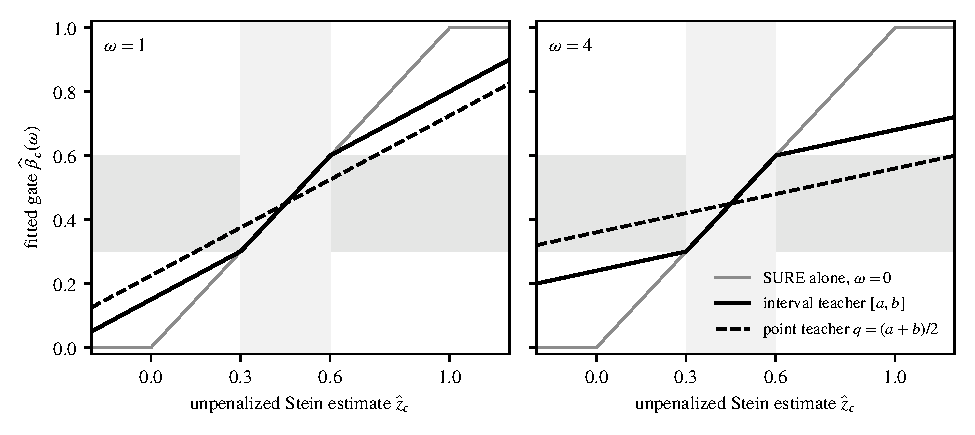
\includegraphics[width=\linewidth]{Figs/theorem1_schematic.pdf}
\caption{Cell solution \eqref{eq:cellsolution} for the interval $[a,b]=[0.3,0.6]$ (shaded)
and for a point teacher at its midpoint $q=0.45$, against the unpenalized Stein estimate
$\widehat z_c$, with penalty weights $\omega=1$ and $\omega=4$. The grey line is SURE alone.}
\label{fig:thm1}
\end{figure}

\begin{remark}[Estimated intervals]\label{rem:estimated}
Theorem~\ref{thm:valid} is deterministic given the interval: it concerns a realized interval
that contains the population target of the cell. Correct bounds on the flip rates make the
population bracket valid, but a teacher estimated from finite pilot data, through a fitted
label-rate curve, can still miss the target. Pointwise confidence limits for the label rate
give pointwise, not simultaneous, coverage over the cells, so for an estimated teacher the
guarantee holds with a probability that the coverage of the realized intervals measures;
simultaneous bands would give a single high-probability statement over all cells.
Sections~\ref{sec:simplan} and~\ref{subsec:bams-gate2} report this coverage, and how often and by
how much the estimated teacher increased risk.
\end{remark}

\begin{corollary}[Bias of a misplaced interval]\label{cor:bias}
Let the interval be common to the cell and let $z_c\in[0,1]$. In the population limit
$\widehat z_c\to z_c$, the penalized gate satisfies
$|\beta_c(\omega)-p_c^\star|=\omega\dist(p_c^\star,[a,b])/(1+\omega)$.
\end{corollary}

\begin{proof}
With $z_c=p_c^\star$, \eqref{eq:cellsolution} moves $p_c^\star$ toward its projection by the
fraction $\omega/(1+\omega)$ of the distance, and no clipping occurs because both points
lie in $[0,1]$.
\end{proof}

A point teacher equal to the midpoint of a valid interval incurs the bias
$\omega|q-p^\star_c|/(1+\omega)$ of \eqref{eq:pointteacher} even when the interval is
correct, whereas the interval teacher incurs none. The penalty weight therefore governs
robustness to misplaced intervals rather than efficiency under valid ones: under a valid
interval $\omega=\infty$ is best on every sample, and cross-fitted SURE guards against
misplacement (Section~\ref{sec:simplan}). The price of an interval is efficiency: where the
Stein estimate already falls inside a wide interval, the interval teacher does nothing, whereas
a point teacher still reduces variance if its target happens to be accurate. For general affine gates with overlapping
basis functions the pathwise property need not hold, and Theorem~\ref{thm:valid} serves as
a benchmark for the simulations.

\subsection{Constructing a context-level interval from membership labels}\label{sec:construct}

To apply Theorem~\ref{thm:valid}, the teacher interval must be a statement about the
context-level target $p^\star$. Membership labels yield such a statement through the prior
inclusion probability. Let the model of Section~\ref{sec:membership} hold, with the noisy
label $\widetilde L_i$ of $H_i$ satisfying $\rho_0(x)\le\bar\rho_0$ and $\rho_1(x)\le
\bar\rho_1$ for all $x$, and let $\widetilde\eta_U(u)=P(\widetilde L=1\mid U=u)$.

\begin{proposition}[Context-level bracket]\label{prop:ctxbracket}
Under these assumptions,
\begin{equation}\label{eq:pibracket}
\pi_-(u)=\frac{\widetilde\eta_U(u)-\bar\rho_0}{1-\bar\rho_0}\le\pi(u)\le
\frac{\widetilde\eta_U(u)}{1-\bar\rho_1}=\pi_+(u).
\end{equation}
Let the slab law and the noise law be fixed, let the endpoints be the posterior means at
inclusion probabilities $\pi_{\rm lo}<\pi_{\rm hi}$ with $\pi_{\rm lo}\le\pi(u)\le\pi_{\rm hi}$,
and let $\zeta(\pi)=\E_\pi\{B(\theta-A)\}/\E_\pi(B^2)$ be the context-level Stein target when the
inclusion probability equals $\pi$. With $t=(\pi-\pi_{\rm lo})/(\pi_{\rm hi}-\pi_{\rm lo})$,
$V_{\rm lo}=\E_{\pi_{\rm lo}}(B^2)$ and $V_{\rm hi}=\E_{\pi_{\rm hi}}(B^2)$,
\begin{equation}\label{eq:zetaclosed}
\zeta(\pi)=\frac{t\,V_{\rm hi}}{(1-t)V_{\rm lo}+t\,V_{\rm hi}},
\end{equation}
which increases from $0$ to $1$ on $[\pi_{\rm lo},\pi_{\rm hi}]$ whenever the endpoint rules
differ with positive probability. Consequently the cell interval
\begin{equation}\label{eq:cellinterval}
I_c=\Bigl[\inf_{u\in c}\zeta\{\pi_-(u)\vee\pi_{\rm lo}\},\
\sup_{u\in c}\zeta\{\pi_+(u)\wedge\pi_{\rm hi}\}\Bigr]
\end{equation}
contains $p^\star_c$, so the teacher is valid on every cell.
\end{proposition}

\begin{proof}
Averaging the pointwise inequalities $(1-\bar\rho_1)\eta(x)\le\widetilde\eta(x)\le
\bar\rho_0+(1-\bar\rho_0)\eta(x)$ over $D$ given $U=u$, and using
$\E\{\eta(X)\mid U=u\}=\pi(u)$, gives \eqref{eq:pibracket}. The joint law of $(\theta,D)$ given
$U=u$ is the mixture $(1-\pi)P_0+\pi P_1$ of the spike and slab laws, so for fixed endpoint
functions both $\E_\pi\{B(\theta-A)\}$ and $\E_\pi(B^2)$ are affine in $\pi$, hence in $t$. At
$\pi=\pi_{\rm lo}$ the posterior mean equals $A$, so $\E\{B(\theta-A)\}=\E\{B(m-A)\}=0$; at
$\pi=\pi_{\rm hi}$ it equals $C=A+B$, so $\E\{B(\theta-A)\}=V_{\rm hi}$. The numerator is
therefore $tV_{\rm hi}$ and the denominator $(1-t)V_{\rm lo}+tV_{\rm hi}$, which gives
\eqref{eq:zetaclosed}; its derivative in $t$ is $V_{\rm lo}V_{\rm hi}/\{(1-t)V_{\rm lo}+tV_{\rm
hi}\}^2>0$. The context-level target is $\zeta\{\pi(u)\}$, and the cell target $z_c$ is a ratio
of averages over $u\in c$ of the numerator and the positive denominator, so it lies between the
smallest and largest pointwise ratios, which monotonicity places within \eqref{eq:cellinterval}.
Since $z_c\in[0,1]$, $p^\star_c=z_c$.
\end{proof}

The map \eqref{eq:zetaclosed} holds for any fixed slab law, Gaussian or double-exponential, and
requires only the two constants $V_{\rm lo}$ and $V_{\rm hi}$, which one-dimensional quadrature
supplies. It depends on the slab law and on $\sigma$, which in practice are estimated, for
instance by marginal maximum likelihood \citep{johnstone2005empirical}; Section~\ref{sec:stress}
examines the effect of a misestimated slab scale. The label rate $\widetilde\eta_U$ is replaced
in practice by confidence limits (Remark~\ref{rem:estimated}). If an estimated bracket lies
entirely outside $[\pi_{\rm lo},\pi_{\rm hi}]$, both ends are clipped to the nearest endpoint
inclusion probability and the interval collapses to the corresponding end of the gate scale.

\section{Known-prior simulation}\label{sec:simplan}

The first study asks whether weak labels with uncertain reliability improve a
Stein-calibrated gate, and by how much, as the training sample grows. It uses a
coefficient-sequence model with a known contextual prior, so that every population quantity,
including the risk of each fitted gate, is computed exactly by quadrature rather than estimated
on test data. The endpoints and the context features are the same for all methods, so
differences reflect only the use of labels.

\subsection{Design}

For $i=1,\ldots,n$, draw a context covariate $U_i\sim{\rm Uniform}(0,1)$, a membership
indicator $H_i\sim{\rm Bernoulli}\{\pi(U_i)\}$ with $\logit\pi(u)=-4+5u$, so that $\pi(u)$
ranges from $0.018$ to $0.731$, a coefficient $\theta_i=0$ if $H_i=0$ and
$\theta_i\sim N(0,\tau^2)$ if $H_i=1$, and $D_i=\theta_i+Z_i$ with $\sigma=1$ and
$\tau\in\{2,4\}$. The exogenous covariate $U_i$ abstracts the role of a parent magnitude or
neighbourhood summary while keeping the oracle computable. The endpoints are the
spike-and-slab rules with $\pi_{\rm lo}=0.01$ and $\pi_{\rm hi}=0.9$, which bracket $\pi(u)$,
and the gate is constant on $K=10$ equal-width cells of $u$, the setting of
Theorem~\ref{thm:valid}. Table~\ref{tab:poprisk} gives the population risks of the reference
rules. Restricting the gate to context costs $0.022$ ($\tau=2$) and $0.035$ ($\tau=4$) relative
to the Bayes rule, while the fixed midpoint and the endpoints are far worse.

\begin{table}[htbp]
\centering
\caption{Exact population risk per coordinate in the known-prior design ($\sigma=1$),
computed by quadrature. The context-only oracle gate is constant on each of the ten cells.}
\label{tab:poprisk}
\begin{tabular}{lccccc}
\toprule
 & Bayes rule & Context-only oracle gate & Midpoint, $p=1/2$ & Endpoint $A$ & Endpoint $C$\\
\midrule
$\tau=2$ & 0.3295 & 0.3516 & 0.4155 & 0.5877 & 0.6025\\
$\tau=4$ & 0.3843 & 0.4190 & 0.4958 & 0.6812 & 0.7411\\
\bottomrule
\end{tabular}
\end{table}

Weak labels come from an independent pilot sample of $5000$ coordinates. Each carries a
noisy membership label $\widetilde L_i$ generated from $H_i$ with instance-dependent flip
probabilities $\rho_1(x)=\bar\rho_1\exp(-d^2/8)$ and $\rho_0(x)=\bar\rho_0\{1-\exp(-d^2/8)\}$,
so that weak signals are missed and large noise coefficients are labelled as signal, with
$(\bar\rho_0,\bar\rho_1)\in\{(0.05,0.20),(0.10,0.30)\}$. The analyst assumes bounds
$k(\bar\rho_0,\bar\rho_1)$ with $k=1$ (exact), $k=1.5$ (conservative), $k=0.5$ (too narrow)
and $k=0$ (labels treated as clean). The teacher fits $\widetilde\eta_U$ by logistic regression
of $\widetilde L$ on a cubic truncated-power spline in $u$ with knots at $0.25$, $0.5$ and $0.75$
(seven coefficients, maximum likelihood by Newton's method). Pointwise $95\%$ limits are
$\logit^{-1}(\widehat\ell\pm1.96\,\widehat{\rm se})$, with $\widehat\ell$ the fitted logit and
$\widehat{\rm se}$ from the inverse observed information. The limits are converted into cell
intervals by \eqref{eq:pibracket}, \eqref{eq:zetaclosed} and \eqref{eq:cellinterval}, with the
infimum and supremum taken over a grid of $40$ points in each cell. We call the point at the
midpoint of this interval the \emph{midpoint teacher}. With $k=0$ the interval does not collapse
to a point: the confidence limits and the variation of $\pi(u)$ within a cell both contribute
width. This differs from the \emph{rate-as-inclusion} teacher of Sections~\ref{sec:stress}
and~\ref{subsec:bams-gate2}, which treats the plug-in label rate as the inclusion probability and
maps it to a single gate value per cell.

The training sample has $n\in\{128,512,2048,8192\}$ coefficients, about $13$ to $820$ per cell.
For every combination of $\tau$, flip bounds and $n$ we draw $500$ replicates; within a
replicate all methods share the training data and the pilot labels. The methods are SURE alone
($\omega=0$), the interval teacher with $\omega\in\{0.25,1,4,\infty\}$ and with $\omega$ chosen by
two-fold cross-fitted SURE over $\{0,0.25,1,4,\infty\}$, and the point teacher with the same
choices. We also evaluate two rules that use labels without the Stein score and are not
restricted to context: the weak-label midpoint rule of Proposition~\ref{prop:midpoint}, with
$\widetilde\eta(x)$ fitted by logistic regression on the spline in $u$ and $d^2$, and forward
correction of that fit with the true flip functions.

Cross-fitting splits the training coefficients at random into two halves. For each candidate
$\omega$, the cell gates are fitted on one half by \eqref{eq:cellsolution} and scored on the
other by the Stein quadratic $\sum_i(V_i\beta_{c(i)}^2-2Y_i\beta_{c(i)})$, which is unbiased
for the risk difference from $A$ because the gate is frozen; the scores of the two directions are
added, the minimizing $\omega$ is selected, and the gate is refitted on all training
coefficients. A cell, or a half-sample cell, with $\sum_iV_i=0$ has no Stein information; its
unpenalized estimate is set to $1/2$ before projection, and an empty scoring cell contributes
zero. Risks of fitted gates are computed exactly as $\sum_c(\mathcal V_c\beta_c^2-2\mathcal
Y_c\beta_c)$ plus a constant, where $\mathcal V_c$ and $\mathcal Y_c$ are the population
contributions of cell $c$ to $\E(V)$ and $\E(Y)$, obtained by quadrature over $u$ and $d$. The
scripts \texttt{sim7.py}, \texttt{sim7\_pointwise.py} and \texttt{stress.py} reproduce all tables
and figures of this section.

\subsection{Results}

The implementation respected Theorem~\ref{thm:valid} wherever its premise held: in all
$64{,}000$ replicate-level checks, covering $\omega\in\{1,\infty\}$, every factor combination and
every assumed bound, no cell whose realized interval contained its target had larger risk under
the interval teacher than under SURE alone. Because the teacher is estimated, the premise can
fail, so we also report how often the fitted teacher increased total risk. With admissible or
conservative bounds this never happened; with bounds that were too narrow or with labels treated
as clean, the interval teacher was worse than SURE alone in at most $1.5\%$ of replicates, by at
most $0.74\times10^{-3}$. The midpoint teacher was worse than SURE alone in $1.5$--$5\%$ of
replicates under the milder noise and in $9$--$16\%$ under the noisier labels, by up to
$4.5\times10^{-3}$, mostly at $n\ge2048$. Table~\ref{tab:sim7} and Figure~\ref{fig:sim7}
report excess risk over the context-only oracle gate.

\begin{table}[htbp]
\centering\small
\caption{Excess risk over the context-only oracle gate ($\times10^{-3}$), $\tau=2$, exact
reliability bounds ($k=1$); Monte Carlo standard errors in parentheses, $500$ replicates.}
\label{tab:sim7}
\begin{tabular}{llcccc}
\toprule
Flip bounds & Method & $n=128$ & $n=512$ & $n=2048$ & $n=8192$\\
\midrule
$(0.05,0.20)$ & SURE alone & 62.89 (1.38) & 20.72 (0.45) & 5.74 (0.13) & 1.66 (0.03)\\
 & Interval teacher, $\omega=\infty$ & 13.44 (0.14) & 9.64 (0.14) & 4.63 (0.09) & 1.61 (0.03)\\
 & Interval teacher, cross-fitted $\omega$ & 19.01 (0.75) & 10.23 (0.19) & 4.70 (0.09) & 1.62 (0.03)\\
 & Midpoint teacher, $\omega=4$ & 8.45 (0.32) & 2.25 (0.06) & 1.07 (0.02) & 0.82 (0.02)\\
 & Midpoint teacher, cross-fitted $\omega$ & 10.14 (0.99) & 3.22 (0.23) & 1.40 (0.04) & 0.90 (0.02)\\
\addlinespace
$(0.10,0.30)$ & SURE alone & 60.51 (1.33) & 20.83 (0.43) & 5.91 (0.12) & 1.58 (0.03)\\
 & Interval teacher, $\omega=\infty$ & 22.14 (0.32) & 13.63 (0.24) & 5.31 (0.10) & 1.56 (0.03)\\
 & Interval teacher, cross-fitted $\omega$ & 27.07 (0.83) & 13.96 (0.26) & 5.38 (0.10) & 1.57 (0.03)\\
 & Midpoint teacher, $\omega=4$ & 10.33 (0.40) & 3.61 (0.07) & 2.39 (0.04) & 2.13 (0.03)\\
 & Midpoint teacher, cross-fitted $\omega$ & 11.51 (0.91) & 4.63 (0.18) & 2.90 (0.05) & 1.57 (0.03)\\
\bottomrule
\end{tabular}
\end{table}

\begin{figure}[htbp]
\centering
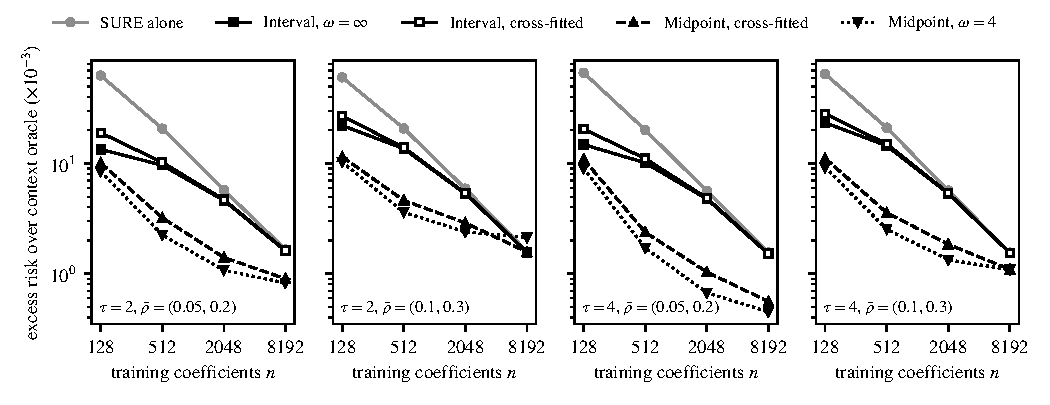
\includegraphics[width=\linewidth]{Figs/sim7_excess.pdf}
\caption{Known-prior simulation: excess risk over the context-only oracle gate against the
number of training coefficients, exact reliability bounds, log scales.}
\label{fig:sim7}
\end{figure}

With few training coefficients the interval teacher removes most of the excess risk of SURE:
with $128$ coefficients and the milder label noise, from $0.0629$ to $0.0134$ at $\omega=\infty$.
The gain shrinks as $n$ grows and is negligible at $n=8192$, where SURE is already close to the
target. With a valid interval the largest penalty is best, as Theorem~\ref{thm:valid} implies;
cross-fitting $\omega$ gives up part of the gain at $n=128$, because half-sample fits sometimes
select small penalties, and its role is protection against misplaced intervals.

The midpoint teacher gains more at every $n$ in the milder setting. With a $5000$-label pilot sample the midpoint lies close to the target, and a
point constrains the gate even where the Stein estimate falls inside the wide admissible interval
(mean width $0.29$ on the gate scale). Its weakness is the bias floor of
\eqref{eq:pointteacher}: with the noisier labels and $\omega=4$ it is worse than SURE alone at
$n=8192$ ($0.00213$ against $0.00158$), whereas the interval teacher is never worse.
Cross-fitting removes that loss on average, though not in every replicate. The same ordering
appeared in the BAMS experiment of Section~\ref{subsec:bams-gate2}. In this design the label
noise is two-sided and interior to the bounds, which places the target near the middle of the
admissible interval and favours the midpoint; Section~\ref{sec:stress} removes that advantage.

\begin{table}[htbp]
\centering\small
\caption{Sensitivity to the assumed reliability bounds, $\tau=2$: coverage of the cell
targets by the teacher intervals (confidence-limit and plug-in versions, $n$-independent),
mean interval width on the gate scale, and excess risk ($\times10^{-3}$) of the cross-fitted
teachers. SURE alone has excess $62.9$ and $20.7$ (milder noise) and $60.5$ and $20.8$
(noisier) at $n=128$ and $512$.}
\label{tab:sim7k}
\begin{tabular}{llrrrrrrr}
\toprule
& & \multicolumn{2}{c}{Coverage (\%)} & & \multicolumn{2}{c}{$n=128$} & \multicolumn{2}{c}{$n=512$}\\
\cmidrule(lr){3-4}\cmidrule(lr){6-7}\cmidrule(lr){8-9}
Flip bounds & $k$ & limits & plug-in & Width & Interval & Midpoint & Interval & Midpoint\\
\midrule
$(0.05,0.20)$ & 0 & 95.3 & 61.1 & 0.157 & 13.51 & 10.02 & 5.52 & 3.48\\
 & 0.5 & 99.9 & 95.7 & 0.223 & 14.99 & 10.37 & 7.91 & 3.38\\
 & 1 & 100.0 & 99.8 & 0.286 & 19.01 & 10.14 & 10.23 & 3.22\\
 & 1.5 & 100.0 & 100.0 & 0.349 & 23.71 & 10.05 & 13.00 & 3.40\\
\addlinespace
$(0.10,0.30)$ & 0 & 77.9 & 41.5 & 0.156 & 13.21 & 11.32 & 6.24 & 4.88\\
 & 0.5 & 99.9 & 94.0 & 0.268 & 19.31 & 12.67 & 9.94 & 4.96\\
 & 1 & 100.0 & 100.0 & 0.373 & 27.07 & 11.51 & 13.96 & 4.63\\
 & 1.5 & 100.0 & 100.0 & 0.480 & 35.74 & 12.29 & 17.47 & 4.69\\
\bottomrule
\end{tabular}
\end{table}

Table~\ref{tab:sim7k} shows the role of the assumed bounds. Conservative bounds keep coverage
at $100\%$ but widen the interval and reduce the gain; bounds that are too narrow, or labels
treated as clean, lose coverage, most clearly with the plug-in teacher ($41.5\%$ for the noisier
labels), and the confidence limits restore much of it. In this design narrow intervals still
helped, because the misplacements were small; Corollary~\ref{cor:bias} bounds the damage in
general.

Secondary runs at $\tau=2$, $n=512$, the milder noise and exact bounds ($250$ replicates)
confirm the pattern. Finer partitions make SURE alone noisier, with excess $12.1$, $21.8$ and
$38.1\times10^{-3}$ for $5$, $10$ and $20$ cells, while the cross-fitted interval teacher stays near
$10\times10^{-3}$ throughout. With only $500$ pilot labels the intervals widen and the interval
teacher gains less ($16.3$ against $21.1$). An affine gate on a linear hat basis, for which
Theorem~\ref{thm:valid} gives no pathwise guarantee, behaves similarly: relative to its own
oracle, excess $17.2$ for SURE alone and $6.8$ for the interval teacher with $\omega=4$.

The two rules that use the labels pointwise in $d$ are in a different class. Fitted to the
$5000$ pilot labels, the weak-label midpoint rule is within $1.2$--$3.2\times10^{-3}$ of the Bayes
risk under exact bounds ($2.0$--$5.7$ under narrow bounds), and forward correction with known
flip functions within $0.9$--$3.3$, over $50$ pilot replicates, well below the context-only floor
of $22$--$35\times10^{-3}$. When membership labels are plentiful and the spike-and-slab model is
trusted, using them directly through Proposition~\ref{prop:midpoint} is therefore preferable.
Stein calibration with a teacher is the tool when the labels are scarce, when the latent model
is only a working model, or when the labels record winners rather than membership.


\subsection{A boundary stress test}\label{sec:stress}

The test places the target near an end of a valid interval. True label noise is one-sided and
attains the analyst's bound: $\rho_0(x)=0$ and $\rho_1(x)=0.30$ for every $x$, so by
Proposition~\ref{prop:bracket} the clean inclusion probability equals the upper end
$\widetilde\eta_U/(1-\bar\rho_1)$ of the bracket. The analyst cannot exclude false positives and
uses the admissible bounds $(\bar\rho_0,\bar\rho_1)=(0.15,0.30)$, or the too-narrow bounds
$(0.075,0.15)$. All other settings are those of Section~\ref{sec:simplan} with $\tau=2$ and $500$
replicates. We compare SURE alone, the interval teacher, the midpoint teacher and the
rate-as-inclusion teacher, the last two with $\omega=4$ and with cross-fitted $\omega$. To probe
the slab model, the analyst also maps the admissible bracket through \eqref{eq:zetaclosed}
computed with a misestimated slab scale, $\tau_a=1.5$ or $\tau_a=3$.

\begin{table}[htbp]
\centering\small
\caption{Boundary stress test, $\tau=2$, admissible bounds. Excess risk over the context-only
oracle gate ($\times10^{-3}$, Monte Carlo SE in parentheses) and, in brackets, the percentage of
replicates in which the method has larger exact risk than SURE alone.}
\label{tab:stress}
\begin{tabular}{lcccc}
\toprule
Method & $n=128$ & $n=512$ & $n=2048$ & $n=8192$\\
\midrule
SURE alone & 64.20 (1.52) & 20.73 (0.50) & 5.77 (0.12) & 1.62 (0.03)\\
Interval teacher, $\omega=\infty$ & 29.52 (0.67) [0] & 13.24 (0.35) [0] & 4.48 (0.10) [0] & 1.50 (0.03) [0]\\
Interval teacher, cross-fitted & 33.76 (1.00) [0] & 13.99 (0.38) [0] & 4.59 (0.10) [0] & 1.52 (0.03) [0]\\
Midpoint teacher, $\omega=4$ & 18.79 (0.45) [0] & 11.26 (0.13) [13] & 9.61 (0.07) [91] & 9.25 (0.06) [100]\\
Midpoint teacher, cross-fitted & 21.91 (0.85) [2] & 13.36 (0.25) [18] & 6.54 (0.15) [42] & 1.82 (0.05) [47]\\
Rate-as-inclusion, $\omega=4$ & 15.21 (0.42) [0] & 8.17 (0.11) [4] & 6.71 (0.05) [67] & 6.38 (0.04) [100]\\
Rate-as-inclusion, cross-fitted & 19.64 (0.98) [0] & 10.32 (0.23) [10] & 5.71 (0.11) [39] & 1.80 (0.05) [43]\\
\bottomrule
\end{tabular}
\end{table}

Table~\ref{tab:stress} shows the trade-off that the theory predicts. The admissible intervals
covered the cell targets in $99.9\%$ of cells, with mean width $0.39$, and the midpoint lay on
average $0.11$ from the target. With $128$ coefficients both point teachers still gain more than
the interval teacher, because their variance reduction outweighs their bias. From $n=2048$ on the
ordering reverses: the interval teacher is never worse than SURE alone and improves on it, the
point teachers with $\omega=4$ are worse than SURE alone in most replicates, and even with
cross-fitted $\omega$ they are worse than SURE alone in $39$--$47\%$ of replicates and on average
($1.80$--$1.82$ against $1.62\times10^{-3}$ at $n=8192$), while the interval teacher reaches
$1.50$. Cross-fitting cannot detect a bias that is small relative to the noise of a half-sample
risk estimate, and at large $n$ such a bias dominates. With the too-narrow bounds coverage fell
to $86\%$; the interval teacher still improved on SURE alone on average at every $n$ (for
example $1.16$ against $1.62\times10^{-3}$ at $n=8192$) but was worse in $8\%$ of replicates at
$n=8192$, as Corollary~\ref{cor:bias} allows. Misestimating the slab scale had little effect:
with $\tau_a=1.5$ or $3$ coverage remained $99.9\%$, and the interval teacher's excess risk changed
by at most $0.35\times10^{-3}$ at every $n$, because the map \eqref{eq:zetaclosed} depends on the
slab only through the ratio $V_{\rm hi}/V_{\rm lo}$.

The interval teacher is therefore best understood as a conditional safeguard. When the interval
is valid it cannot hurt, and it helps most when training data are scarce and the interval is
narrow. Its cost, relative to a point teacher whose target happens to be accurate, is
efficiency. A point teacher can gain more, but its bias does not vanish with more data and is
not reliably detected by cross-fitting.

\section{Wavelet experiments with two BAMS rules}\label{sec:waveplan}

Bayesian adaptive multiresolution shrinkage (BAMS) uses a level-dependent
spike-and-slab prior for wavelet detail coefficients \citep{vidakovic2001bams}.
At level $j$, write the prior as
$$
\theta\sim\epsilon_j\delta_0+(1-\epsilon_j)\,\mathrm{DE}(0,\tau_j),
\qquad f_{\mathrm{DE}}(t;\tau_j)=\frac{1}{2\tau_j}\exp(-|t|/\tau_j).
$$
Here $\epsilon_j$ is the probability of the spike at zero, and $\tau_j$ is the
scale of the double-exponential slab. Let $f_0(d)$ and $f_{1j}(d)$ denote the
marginal observation densities under the spike and slab, respectively, and
let $m_{1j}(d)$ denote the conditional mean given slab membership. The
posterior-mean rule is
$$
\delta_j(d)=m_{1j}(d)
\frac{(1-\epsilon_j)f_{1j}(d)}
     {\epsilon_j f_0(d)+(1-\epsilon_j)f_{1j}(d)}.
$$
The first experiment varies $\tau_j$ and studies labels of the better
shrinkage action. The second varies $\epsilon_j$ and studies labels of slab
membership. Both use length-$1024$ signals, an orthonormal wavelet
representation, and independent Gaussian observation noise of standard
deviation one. We pass the eight scaling coefficients through unchanged.
By Parseval's identity, the weighted sum over levels of the coefficient
squared errors, divided by $1024$, is the signal-domain MSE. AMSE averages
this quantity across the test realizations.

\subsection{BAMS gate 1: slab-scale endpoints and noisy winner labels}
\label{subsec:bams-gate1}

We use the Doppler signal and the periodic Symmlet~4 transform with detail
levels $j=3,\ldots,9$. With $t_i=i/n$, the unscaled signal is
$\sqrt{t_i(1-t_i)}\sin\{2.1\pi/(t_i+0.05)\}$. We rescale it so that its
sample standard deviation divided by the noise standard deviation is~$5$
(root SNR, equivalent to a variance ratio of~$25$ under this convention).
We train on $20$ independent noisy realizations of the fixed clean signal
and evaluate on $100$ fresh noisy realizations. For training methods that
use pairs, each training input comes with an independent second noisy
realization. The experiment is a controlled illustration of Sections~\ref{sec:setting}
to~\ref{sec:stein}, namely of winner labels, cost weighting and the Stein score, and it does not
use the interval teacher. Its repeated-measurement design is chosen because it supplies a genuine
independent noisy view, and hence genuine noisy winner labels; it is not a proposed workflow, since
an analyst with replicates of one fixed signal could also average them, and it does not test
transfer of a fitted gate to unseen signals.

For each first observation we apply the original BAMS nuisance-parameter
calibration, including its working double-exponential observation
likelihood. At each level we evaluate two versions of the BAMS rule,
using $0.3\tau_j$ and $3\tau_j$ with the fitted observation model and
$\epsilon_j$ held fixed. The smaller-magnitude output is $A_i$ and the
larger is $C_i$, so the gate weight on $C_i$ always represents weaker
shrinkage, on either side of zero. The candidate estimate is
$A_i+(C_i-A_i)p_j(X_i)$. The relatively wide slab-scale pair provides
visibly distinct actions in the intermediate range of coefficient
magnitudes (Figure~\ref{fig:bams1-rules}).

\begin{figure}[!htbp]
\centering
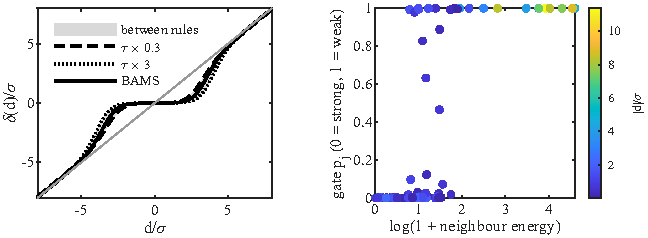
\includegraphics[width=.96\linewidth]{Figs/BAMS2gate1_tau03_30_rules.pdf}
\caption{BAMS gate 1. Left: levelwise BAMS curves at slab scales
$0.3\tau_j$ and $3\tau_j$, with the reference BAMS rule and the identity.
The shaded region is the action interval. Right: fitted context-only SURE
gate against neighbouring energy, with colour indicating the standardized
coefficient magnitude. Each point is a level-$7$ coefficient in a single
test realization.}
\label{fig:bams1-rules}
\end{figure}

We fit level-specific logistic gates with a ridge penalty. The features
are log-transformed standardized energies of the observed coefficient,
the two neighbours at its level, the parent, and the two children. We
compare a constant gate, magnitude-only gates, and combinations of the
context features. The paired-replicate fit minimizes squared error
against the second observation. Specifically, if $T_i$ denotes the
replicate coefficient, its objective has quadratic weight $B_i^2$ and
linear score $B_i(T_i-A_i)$, where $B_i=C_i-A_i$. The replicate's independent,
mean-zero noise adds only a constant to the expected squared error.
The SURE fit uses the score of Proposition~\ref{prop:score}, either with a
constant gate or with context excluding the current coefficient. In this
experiment the derivative holds the data-dependent BAMS nuisance estimates
fixed, so the resulting SURE score is a plug-in approximation. We also
fit this context gate directly to each test signal to assess the case with
only one realization available.

The replicate's winning-rule label is
$\mathbf{1}\{\widehat r_i>0\}$, where
$\widehat r_i=(T_i-A_i)^2-(T_i-C_i)^2$ is the observed analogue of
\eqref{eq:contrast}. The two vote fits use identical features and logistic
loss, with unit weights or weights $|\widehat r_i|$. Both fitted scores
are used as interpolation gates. Lemma~\ref{lem:cost} explains the
importance of the cost weighting for a binary decision. Here the two
soft gates let us examine its practical effect on reconstruction.
Figure~\ref{fig:bams1-votes} shows that agreement with the clean-signal
winner is near chance for the smallest magnitudes. In this range the
actions often nearly coincide, so a disagreement can have little effect
on loss. Accuracy alone gives those votes the same importance as votes
with a large cost contrast.

\begin{figure}[!htbp]
\centering
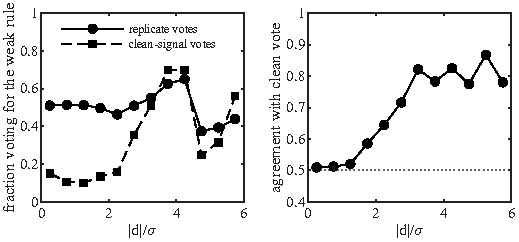
\includegraphics[width=.94\linewidth]{Figs/BAMS2gate1_tau03_30_votes.pdf}
\caption{BAMS gate 1. Left: the fraction of training coefficients voting
for the weak rule in each magnitude bin, using the independent noisy
replicate and the clean signal. Right: agreement between the two votes.
The horizontal reference marks chance-level agreement.}
\label{fig:bams1-votes}
\end{figure}

\begin{table}[!htbp]
\centering
\small
\caption{BAMS gate 1 on Doppler. $\Delta$ is the AMSE difference from reference BAMS. SE is the paired Monte Carlo standard error for $\Delta$.}
\label{tab:bams1-risk}
\begin{tabular}{lrrr}
\toprule
Method & AMSE & $\Delta$ & SE \\
\midrule
Reference BAMS & 0.16487 & 0.00000 & 0.00000 \\
BAMS, $0.3\tau_j$ & 0.16086 & -0.00401 & 0.00066 \\
BAMS, $3\tau_j$ & 0.18236 & 0.01749 & 0.00076 \\
Midpoint & 0.16536 & 0.00048 & 0.00017 \\
Pair, constant & 0.15745 & -0.00742 & 0.00051 \\
Pair, magnitude & 0.15660 & -0.00828 & 0.00051 \\
Pair, magnitude and neighbours & 0.14899 & -0.01588 & 0.00043 \\
Pair, magnitude and multiscale context & 0.14610 & -0.01878 & 0.00050 \\
Pair, context only & 0.14542 & -0.01945 & 0.00039 \\
SURE, constant & 0.15690 & -0.00797 & 0.00050 \\
SURE, context only & 0.14470 & -0.02018 & 0.00040 \\
SURE, fitted on one test signal & 0.15389 & -0.01098 & 0.00044 \\
Votes, unweighted & 0.16056 & -0.00431 & 0.00017 \\
Votes, cost-weighted & 0.14913 & -0.01574 & 0.00031 \\
Coefficientwise projection oracle & 0.13506 & -0.02981 & 0.00040 \\
\bottomrule
\end{tabular}
\end{table}

The context-only SURE gate is the best fitted method in
Table~\ref{tab:bams1-risk}. It reduces AMSE from $0.16487$ for reference BAMS
to $0.14470$, a $12.2\%$ reduction, and lowers AMSE by $0.01616$ relative to the
better individual endpoint. The midpoint gives $0.16536$, so the availability
of two distant rules alone achieves little. Adding neighbourhood energy
to the magnitude-only paired gate reduces AMSE from $0.15660$ to $0.14899$;
adding parent and child energies reduces it further to $0.14610$. The
context-only paired gate reaches $0.14542$. Cost weighting improves the
vote fit from $0.16056$ to $0.14913$, whereas the unweighted gate barely
improves on the better endpoint ($0.16086$). The clean coefficientwise
projection reaches $0.13506$ and supplies a lower benchmark for this
action interval. Figure~\ref{fig:bams1-amse} reports differences on the
common test realizations.

\begin{figure}[!htbp]
\centering
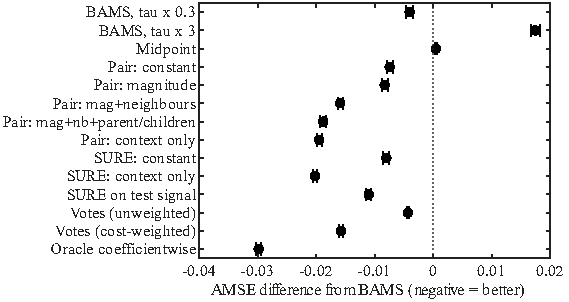
\includegraphics[width=.94\linewidth]{Figs/BAMS2gate1_tau03_30_amse.pdf}
\caption{BAMS gate 1. AMSE differences from reference BAMS for the
$0.3\tau_j$ and $3\tau_j$ pair. Bars give one paired Monte Carlo standard
error.}
\label{fig:bams1-amse}
\end{figure}

Training from $20$ realizations improves the context-only SURE result
over fitting on a single signal ($0.14470$ versus $0.15389$). The plug-in SURE score, which holds
the estimated BAMS nuisance parameters fixed, gives slightly lower AMSE than the paired-replicate
fit ($0.14470$ against $0.14542$, a difference of about two paired standard errors), so we see no
sign that the plug-in approximation harms the fitted gate here.
The wider action interval is useful because the gate learns when to
use it. The poorer of the two endpoints has AMSE $0.18236$, so choosing
weak shrinkage indiscriminately would worsen reconstruction.

\subsection{BAMS gate 2: spike-probability endpoints and the interval teacher}
\label{subsec:bams-gate2}

We generate independent signals directly in orthonormal wavelet
coordinates. At each level, two equal-sized blocks define quiet and active
contexts $u$. The observed block identity is available to the estimator.
Draw $H_i\mid j,u\sim\mathrm{Bernoulli}\{\pi_j(u)\}$, set $\theta_i=0$ for
$H_i=0$, and draw $\theta_i\sim\mathrm{DE}(0,\tau_j)$ for $H_i=1$.
The Gaussian observation model and the rule parameters are fixed in this
experiment, so the Stein identity applies directly. We use the BAMS
spike and DE slab with a Gaussian observation likelihood. The design is
given in Table~\ref{tab:bams2-design}. No realization is rescaled.
The root expected signal power divided by the noise standard deviation
is $0.921$, computed as
$\{n^{-1}\sum_j 2^j\tau_j^2[\pi_j(\mathrm{quiet})+
\pi_j(\mathrm{active})]\}^{1/2}/\sigma$.
The quiet and active contexts share a slab scale at each level, and
differ in how often a signal coefficient occurs.

\begin{table}[!htbp]
\centering
\small
\caption{BAMS gate 2 design. The spike weights define the endpoint rules. The two true inclusion probabilities define the quiet and active blocks.}
\label{tab:bams2-design}
\begin{tabular}{rrrrrr}
\toprule
$j$ & $\tau_j$ & $\epsilon_{j,\mathrm{strong}}$ & $\epsilon_{j,\mathrm{weak}}$ & $\pi_j(\mathrm{quiet})$ & $\pi_j(\mathrm{active})$ \\
\midrule
3 & 2.800 & 0.940 & 0.500 & 0.100 & 0.380 \\
4 & 2.533 & 0.943 & 0.513 & 0.095 & 0.363 \\
5 & 2.267 & 0.947 & 0.527 & 0.090 & 0.347 \\
6 & 2.000 & 0.950 & 0.540 & 0.085 & 0.330 \\
7 & 1.733 & 0.953 & 0.553 & 0.080 & 0.313 \\
8 & 1.467 & 0.957 & 0.567 & 0.075 & 0.297 \\
9 & 1.200 & 0.960 & 0.580 & 0.070 & 0.280 \\
\bottomrule
\end{tabular}
\end{table}

At level $j$, let $\pi_{j,\rm lo}=1-\epsilon_{j,\mathrm{strong}}$ and
$\pi_{j,\rm hi}=1-\epsilon_{j,\mathrm{weak}}$. The two endpoints bracket the
true inclusion probability in both contexts. Increasing inclusion
increases the posterior slab probability for every $d$, so it weakens
shrinkage. In a separate pilot sample of four signals, the membership
labels have false-positive rate $0.04$ and false-negative rate $0.16$.
Only the corrupted label is observed. We estimate its positive rate
within each level and context, and use pointwise $95\%$ Wilson limits
$q_-$ and $q_+$. By Proposition~\ref{prop:bracket}, upper flip bounds
$(\bar\rho_0,\bar\rho_1)$ give an inclusion interval with ends
$(q_--\bar\rho_0)/(1-\bar\rho_0)$ and $q_+/(1-\bar\rho_1)$, each clipped
to $[\pi_{j,\rm lo},\pi_{j,\rm hi}]$. We use admissible bounds $(0.05,0.20)$ and
narrow bounds $(0.025,0.10)$ as a sensitivity check. The point teacher here is the
rate-as-inclusion teacher: it treats the observed pilot rate as the inclusion probability and
maps it to a single gate value per cell, unlike the midpoint teacher of
Section~\ref{sec:simplan}.

The needed interval is on the scale of the context gate. Proposition~\ref{prop:ctxbracket}
applies with the double-exponential slab: at level $j$ the map \eqref{eq:zetaclosed} holds with
$\pi_{j,\rm lo}$, $\pi_{j,\rm hi}$ and constants $V_{\rm lo},V_{\rm hi}$ computed by
one-dimensional quadrature, and it transforms each inclusion bound into the corresponding gate
bound. The context oracle uses $\zeta_j\{\pi_j(u)\}$, and the full Bayes oracle uses the
posterior mean at the true inclusion probability of the cell.

We fit one gate per level and context to an independent training sample
of either one or $20$ length-$1024$ signals. The teacher is frozen during
the fit. The unconstrained SURE target for a cell is the ratio of the
summed linear Stein scores to the summed squared action separations.
The interval penalty in \eqref{eq:objective}, with $\omega=4$, moves
this ratio toward the nearest point of the interval when it is outside.
We then clip the gate to $[0,1]$. The point teacher uses the same
penalty with a singleton target. We compare the fitted gates with both
endpoints, the midpoint, a reference rule at the pooled level inclusion
probability, and the two oracles. We repeat the experiment $200$ times
with $12$ independent test signals per repeat, shared across methods
and training sizes.

\begin{figure}[!htbp]
\centering
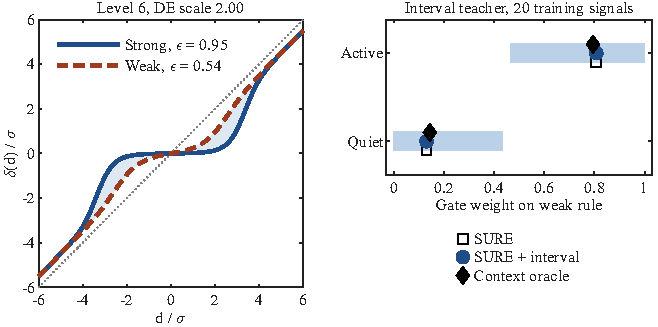
\includegraphics[width=\linewidth]{Figs/BAMS2gate2_rules_teacher.pdf}
\caption{BAMS gate 2 at level $6$. Left: BAMS-type posterior means with
a common DE scale and different spike probabilities. Right: the two
teacher intervals and the fitted and oracle gates in one repetition with
$20$ training signals. The bands denote the admissible-bound intervals.}
\label{fig:bams2-teacher}
\end{figure}

\begin{table}[!htbp]
\centering
\small
\caption{BAMS gate 2 risk. Each $\Delta$ is relative to SURE alone at the same training size, with paired Monte Carlo SE in parentheses. Differences and SEs are in units of $10^{-3}$.}
\label{tab:bams2-risk}
\begin{tabular}{lrrrr}
\toprule
& \multicolumn{2}{c}{One training signal} & \multicolumn{2}{c}{20 training signals} \\\cmidrule(lr){2-3}\cmidrule(lr){4-5} Method & AMSE & $\Delta$ (SE) & AMSE & $\Delta$ (SE) \\
\midrule
Strong endpoint & 0.28347 & 35.963 (0.411) & 0.28347 & 43.787 (0.311) \\
Weak endpoint & 0.28100 & 33.492 (0.356) & 0.28100 & 41.316 (0.226) \\
Midpoint & 0.25111 & 3.604 (0.307) & 0.25111 & 11.428 (0.135) \\
Reference BAMS-type & 0.24897 & 1.467 (0.307) & 0.24897 & 9.291 (0.137) \\
SURE alone & 0.24751 & 0.000 (0.000) & 0.23968 & 0.000 (0.000) \\
SURE + point teacher & 0.24079 & -6.719 (0.264) & 0.23971 & 0.023 (0.048) \\
SURE + interval teacher & 0.24427 & -3.243 (0.204) & 0.23967 & -0.015 (0.004) \\
SURE + narrow interval teacher & 0.24329 & -4.214 (0.223) & 0.23961 & -0.074 (0.009) \\
Context oracle & 0.23900 & -8.510 (0.300) & 0.23900 & -0.686 (0.039) \\
Bayes oracle & 0.23819 & -9.316 (0.301) & 0.23819 & -1.491 (0.055) \\
\bottomrule
\end{tabular}
\end{table}

\begin{table}[!htbp]
\centering
\small
\caption{Empirical coverage of the context oracle and mean interval width on the gate scale. Each entry gives quiet / active. The point teacher has zero width and zero exact coverage at every level.}
\label{tab:bams2-coverage}
\begin{tabular}{rrrrr}
\toprule
& \multicolumn{2}{c}{Admissible bounds} & \multicolumn{2}{c}{Narrow bounds} \\\cmidrule(lr){2-3}\cmidrule(lr){4-5} Level & Coverage (\%) & Width & Coverage (\%) & Width \\
\midrule
3 & 100.0 / 99.0 & 0.848 / 0.756 & 97.5 / 99.0 & 0.784 / 0.696 \\
4 & 98.5 / 99.0 & 0.737 / 0.644 & 97.0 / 97.0 & 0.660 / 0.575 \\
5 & 98.0 / 99.0 & 0.640 / 0.574 & 97.5 / 98.0 & 0.557 / 0.494 \\
6 & 100.0 / 100.0 & 0.528 / 0.504 & 98.5 / 99.0 & 0.452 / 0.412 \\
7 & 100.0 / 100.0 & 0.485 / 0.450 & 95.5 / 98.0 & 0.394 / 0.335 \\
8 & 100.0 / 100.0 & 0.437 / 0.395 & 96.5 / 99.0 & 0.334 / 0.272 \\
9 & 100.0 / 100.0 & 0.401 / 0.351 & 94.5 / 100.0 & 0.281 / 0.227 \\
\bottomrule
\end{tabular}
\end{table}

\begin{table}[!htbp]
\centering
\small
\caption{Mean fitted gates at level $6$ across the $200$ repetitions. A larger gate places more weight on the weak rule.}
\label{tab:bams2-gates}
\begin{tabular}{lrrrr}
\toprule
& \multicolumn{2}{c}{One training signal} & \multicolumn{2}{c}{20 training signals} \\\cmidrule(lr){2-3}\cmidrule(lr){4-5} Method & Quiet & Active & Quiet & Active \\
\midrule
SURE alone & 0.265 & 0.658 & 0.141 & 0.795 \\
SURE + point teacher & 0.186 & 0.727 & 0.194 & 0.754 \\
SURE + interval teacher & 0.219 & 0.714 & 0.141 & 0.796 \\
SURE + narrow interval teacher & 0.208 & 0.722 & 0.144 & 0.796 \\
Context oracle & 0.143 & 0.794 & 0.143 & 0.794 \\
\bottomrule
\end{tabular}
\end{table}

\begin{figure}[!htbp]
\centering
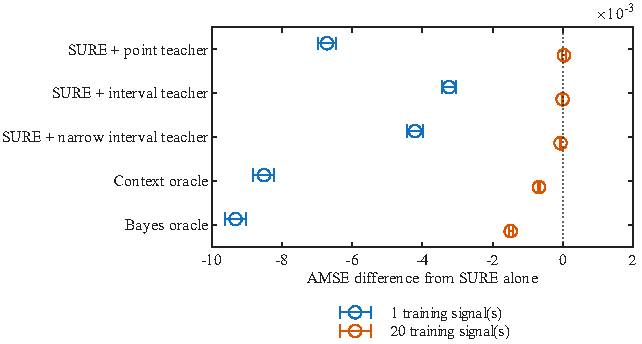
\includegraphics[width=.94\linewidth]{Figs/BAMS2gate2_risk.pdf}
\caption{BAMS gate 2. AMSE differences from SURE alone, with one paired
Monte Carlo standard error. The SURE reference is computed separately
for each training size. The AMSE differences are in units $10^{-3}.$}
\label{fig:bams2-risk}
\end{figure}

With one training signal, the admissible interval teacher improves on
SURE alone by $0.00324$ (paired Monte Carlo SE $0.00020$).
The point teacher gives the lowest AMSE among the fitted gates in this
regime, improving on SURE alone by $0.00672$. The narrow interval falls
between the two. This is consistent with a bias--variance trade-off:
a tighter constraint can stabilize a noisy fit even when its target is
imperfect. Empirical coverage of the context oracle is $98$--$100\%$
for the admissible intervals, compared with $94.5$--$100\%$ for the
narrow intervals and zero exact coverage for the singleton teachers. As in
Section~\ref{sec:simplan}, the rate-as-inclusion teacher gains more than the interval teacher when
the training sample is small and its target is close; Section~\ref{sec:stress} shows the opposite
when the target lies near an end of the interval.
The admissible intervals are wide at the coarsest levels, where
four pilot signals supply only $16$ coefficients per context at level~3.
Their coverage and widths explain why the interval penalty can be
less active than the point penalty. The guarantee of
Theorem~\ref{thm:valid} applies when a realized interval contains the
context oracle. The empirical coverage measurements record how often
that condition holds in each cell.

With $20$ training signals, SURE alone improves from $0.24751$ to
$0.23968$, close to the context oracle at $0.23900$. The admissible
interval teacher changes AMSE by about $-1.5\times10^{-5}$, while the
point teacher's difference from SURE alone is small relative to its
paired Monte Carlo standard error. For example, at level~6 the SURE
gates move from mean quiet and active values $(0.265,0.658)$ with one
training signal to $(0.141,0.795)$ with $20$, close to the oracle
$(0.143,0.794)$. Figure~\ref{fig:bams2-risk} contrasts the two training
regimes. More training coefficients per cell improve learning in this
design, especially where the separation of the two rules is appreciable.
Both experiments keep the signal length fixed; longer individual signals
would supply more coefficients, but their benefit would also depend on
how many fall in each context and on the information they carry.

\section{Discussion}\label{sec:discussion}

The paper separates two roles that are conflated when a classifier is trained on noisy keep
labels. The Stein score measures the reconstruction cost of each action without any label,
and it determines the population target of a context gate. Labels, when they carry
information beyond the features, describe which actions are plausible; with bounded but
unknown reliability they do so through an interval rather than a point. Interval-teacher
calibration combines the two. Its guarantee is conditional but pathwise: an interval that
contains the target cannot hurt a piecewise-constant gate on any sample. Whether an estimated
interval contains the target depends on defensible bounds on the flip rates, on the estimation
of the label rate, and, for the context-level construction, on the slab model, and it holds with a
probability that the observed coverage measures. In our simulations, estimated intervals with
admissible bounds never increased risk, and with too-narrow bounds rarely and slightly; point
teachers gained more when their targets were accurate, but their bias persisted with more data
and was not reliably removed by cross-fitting.

Several limitations remain. The pathwise result does not extend to gates with overlapping
basis functions or to smoothing penalties across cells, for which only convexity and the
population characterization are available. The context-level bracket uses uniform bounds on
the flip rates; instance-dependent bounds can be used pointwise
(Proposition~\ref{prop:bracket}) but do not average as simply. Stein's identity requires known
noise variance and white Gaussian noise; colored noise and redundant transforms require the
covariance in the divergence term and an account of the synthesis operator in the signal-domain
loss. The Doppler experiment shows that context and cost weighting improve reconstruction
for a fixed underlying signal. The membership experiment shows how bounded label
corruption can improve a lightly trained Stein gate, while more training reduces
the contribution of the teacher. Generalization to unseen signal families, sensitivity to
signal length, and an application in which an external detector supplies the labels remain
to be studied.

The results suggest a simple practice. The Stein gate needs no labels and should always be
fitted; when each cell holds many coefficients it is close to its target, and labels add little.
When training data are scarce, labels should be used, and their meaning decides how. Winner
labels need cost weights or, better, replacement by the Stein score. Membership labels should be
turned into intervals with reliability bounds that the analyst can defend; conservative bounds
cost efficiency but not validity, so it is better to err on the wide side, and confidence limits
for the label rate should be used rather than plug-in values. An interval teacher with a large
penalty is then a conditional safeguard: it cannot hurt where its interval is valid, and its
value grows as training data become scarce and the interval narrows. A point teacher can gain
more when the analyst has reason to believe its target is accurate, for instance two-sided noise
well inside the bounds, but it should be reserved for small training samples, because its bias
does not vanish with more data. Finally, when membership labels are plentiful and the
spike-and-slab model is credible, the labels can be used pointwise through the minimax midpoint
rule, which in our simulation came within a few thousandths of the Bayes risk.

\appendix

\section{Margin bounds for binary decisions}\label{app:margin}

For an evaluation region observable in $X_i$, sample a coordinate with probability
proportional to its probability of lying in the region and draw its features conditional on
lying there; call the resulting law $Q$, and let $N$ be the expected number of coordinates in
the region. A fitted score $\widehat g$, independent of the test signal, induces the binary
rule that selects $C_i$ when $\widehat g\ge0$.

\begin{theorem}[Binary margin bounds]\label{thm:margin}
If $Q(0<|g|\le t)\le c_0t^\kappa$ for all $t>0$ and $\|\widehat g-g\|_{L_2(Q)}\le\nu$,
the total excess risk of the plug-in binary rule over the Bayes binary rule on the region is
at most $2Nc_0^{1/(\kappa+2)}\nu^{2(\kappa+1)/(\kappa+2)}$. Without a margin
condition, an $L_1(Q)$ bound $\nu$ gives $N\nu$; with the margin condition,
an $L_\infty(Q)$ bound $\nu$ gives $Nc_0\nu^{\kappa+1}$.
\end{theorem}

\begin{proof}
For each coordinate in the region the loss difference between the two binary actions is
$\pm r_i$, and conditioning on $X_i$ and on the independent fit shows that the excess risk
equals $N\E_Q[|g|\,\ind\{\text{wrong endpoint}\}]$. On a disagreement with $g\ne0$, $\widehat g$
and $g$ have opposite signs, so $|g|\le|\widehat g-g|$. Splitting at $t>0$, the contribution
of $\{0<|g|\le t\}$ is at most $\E_Q[|\widehat g-g|\ind\{0<|g|\le t\}]\le\nu\sqrt{c_0}
t^{\kappa/2}$ by the Cauchy--Schwarz inequality, and the contribution of $\{|g|>t\}$ is at
most $\E_Q|g|^2\ind\{\cdot\}/t\le\nu^2/t$. Choosing $t=(\nu/\sqrt{c_0})^{2/(\kappa+2)}$ gives the first bound. The pointwise inequality gives the $L_1$ bound, and
under a uniform bound disagreement requires $|g|\le\nu$, which gives the last.
\end{proof}

The exponent $2(\kappa+1)/(\kappa+2)$ is the fast plug-in rate of
\citet{audibert2007fast} under the margin condition of \citet{mammen1999smooth} and
\citet{tsybakov2004optimal}. Retaining $|g|$ inside the expectation, rather than bounding the
local cost by a constant, avoids any boundedness assumption on $\theta$ and improves on the
exponent $\kappa/(\kappa+1)$ obtained from an $L_1$ error combined with a uniform cost bound.

\section*{Code availability}
The scripts \texttt{sim7.py}, \texttt{sim7\_pointwise.py}, \texttt{stress.py} and
\texttt{sim7\_report.py} reproduce Section~\ref{sec:simplan}, and the MATLAB scripts \texttt{BAMS2gate1.m} and \texttt{BAMS2gate2.m} reproduce
Section~\ref{sec:waveplan}.

\bibliographystyle{apalike}
\bibliography{MLShrinkNoisyLabels06}

\end{document}
